\documentclass[paper=letter,fontsize=11pt]{scrartcl} % KOMA-article class
							
\usepackage[english]{babel}
\usepackage[utf8x]{inputenc}
\usepackage[protrusion=true,expansion=true]{microtype}
\usepackage{amsmath,amsfonts,amsthm}     % Math packages
\usepackage{graphicx}                    % Enable pdflatex
\usepackage[svgnames]{xcolor}            % Colors by their 'svgnames'
\usepackage{geometry}
	%\textheight=700px                    % Saving trees ;-)
%\usepackage{url}
\usepackage[colorlinks=true,
linkcolor=blue,
urlcolor=blue]{hyperref}
\usepackage{float}
\usepackage{etaremune}
\usepackage{wrapfig}

\usepackage{attachfile}

\frenchspacing              % Better looking spacings after periods
\pagestyle{empty}           % No pagenumbers/headers/footers

%\addtolength{\voffset}{-40pt}
%\addtolength{\textheight}{20pt}

\setlength\topmargin{0pt}
\addtolength\topmargin{-\headheight}
\addtolength\topmargin{-\headsep}
\setlength\oddsidemargin{0pt}
\setlength\textwidth{\paperwidth}
\addtolength\textwidth{-2in}
\setlength\textheight{\paperheight}
%\addtolength\textheight{-3in}
\addtolength\textheight{-2in}
\usepackage{layout}

%%% Custom sectioning}{sectsty package)
%%% ------------------------------------------------------------
\usepackage{sectsty}

\sectionfont{%			            % Change font of \section command
	\usefont{OT1}{phv}{b}{n}%		% bch-b-n: CharterBT-Bold font
	\sectionrule{0pt}{0pt}{-5pt}{3pt}}

%%% Macros
%%% ------------------------------------------------------------
\newlength{\spacebox}
\settowidth{\spacebox}{8888888888}			% Box to align text
\newcommand{\sepspace}{\vspace*{1em}}		% Vertical space macro

\newcommand{\MyName}[1]{ % Name
		\Huge \usefont{OT1}{phv}{b}{n} \hfill #1
		\par \normalsize \normalfont}
		
\newcommand{\MySlogan}[1]{ % Slogan}{optional)
		\large \usefont{OT1}{phv}{m}{n}\hfill \textit{#1}
		\par \normalsize \normalfont}

\newcommand{\NewPart}[2]{\section*{\uppercase{#1} #2}}

\newcommand{\PersonalEntry}[2]{
		\noindent\hangindent=2em\hangafter=0 % Indentation
		\parbox{\spacebox}{        % Box to align text
		\textit{#1}}		       % Entry name}{birth, address, etc.)
		\hspace{1.5em} #2 \par}    % Entry value

\newcommand{\SkillsEntry}[2]{      % Same as \PersonalEntry
		\noindent\hangindent=2em\hangafter=0 % Indentation
		\parbox{\spacebox}{        % Box to align text
		\textit{#1}}			   % Entry name}{birth, address, etc.)
		\hspace{1.5em} #2 \par}    % Entry value	
		
\newcommand{\EducationEntry}[4]{
		\noindent \textbf{#1} \hfill      % Study
		\colorbox{White}{%
			\parbox{6em}{%
			\hfill\color{Black}#2}} \par  % Duration
		\noindent \textit{#3} \par        % School
		\noindent\hangindent=2em\hangafter=0 \small #4 % Description
		\normalsize \par}

\newcommand{\WorkEntry}[4]{				  % Same as \EducationEntry
		\noindent \textbf{#1} \hfill      % Jobname
		\colorbox{White}{\color{White}#2} \par  % Duration
		\noindent \textit{#3} \par              % Company
		\noindent\hangindent=2em\hangafter=0 \small #4 % Description
		\normalsize \par}

\newcommand{\PaperEntry}[7]{
		\noindent #1, ``\href{#7}{#2}", \textit{#3} \textbf{#4}, #5 (#6).}

\newcommand{\ArxivEntry}[3]{
		\noindent #1, ``\href{http://arxiv.org/abs/#3}{#2}", \textit{{cond-mat/}#3}.}
        
\newcommand{\BookEntry}[4]{
		\noindent #1, ``\href{#3}{#4}", \textit{#3}.}
        
\newcommand{\FundingEntry}[5]{
        \noindent #1, ``#2", \$#3 (#4, #5).}

\newcommand{\TalkEntry}[4]{
		\noindent #1, #2, #3 #4}

\newcommand{\ThesisEntry}[5]{
		\noindent #1 -- #2 #3 ``#4" \textit{#5}}

\newcommand{\CourseEntry}[3]{
		\noindent \item{#1: \textbf{#2} \\ #3}}

%%% Begin Document
%%% ------------------------------------------------------------
\begin{document}

%\layout

% you can upload a photo and include it here...
\begin{wrapfigure}{l}{0.5\textwidth}
	\vspace*{-2em}
		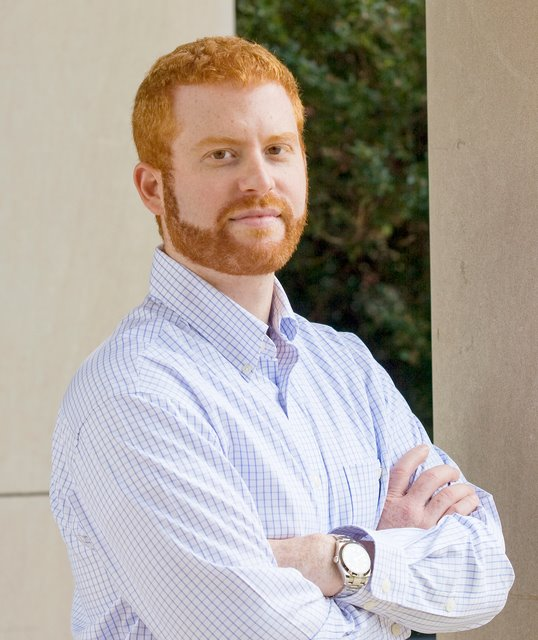
\includegraphics[width=0.2\textwidth]{Appelbaum.JPG}
\end{wrapfigure}

\MyName{Ian Appelbaum}
\MySlogan{\vspace{-0.3in}\begin{flushright}\href{http://maps.google.com/maps/ms?ie=UTF&msa=0&msid=205373386241137011999.000494c753d05031c4fe4}{Physical Sciences Complex}\\University of Maryland, College Park \\
(301) 337-7461\\
\href{mailto:appelbaum@physics.umd.edu}{appelbaum@physics.umd.edu}\\
\href{http://appelbaumlab.umd.edu/CV.html}{http://appelbaum.physics.umd.edu}
\end{flushright}}

%\sepspace
 \NewPart{Overview}{}
 Professor of Physics, APS Fellow, Condensed Matter Experiment {\em and} Theory.
%%% Personal details
%%% ------------------------------------------------------------
% \NewPart{}{}

% \PersonalEntry{Address}{\href{http://maps.google.com/maps/ms?ie=UTF&msa=0&msid=205373386241137011999.000494c753d05031c4fe4}{Physical Sciences Complex}, University of Maryland, College Park}
% \PersonalEntry{Phone}{(301) 337-7461}
% \PersonalEntry{Mail}{\href{mailto:appelbaum@physics.umd.edu}{appelbaum@physics.umd.edu}}
% \PersonalEntry{WWW}{\href{http://appelbaumlab.umd.edu/CV.html}{http://appelbaum.physics.umd.edu}}


%%% Work experience
%%% ------------------------------------------------------------
\NewPart{Appointments}{}

\noindent \textbf{Professor of Physics} \hfill      % Study
		\colorbox{White}{%
			\parbox{6em}{%
			\hfill\color{Black}2016-$\qquad$}} \par

\EducationEntry{\textattachfile[color=1 0 1]{research.pdf}{Associate Professor of Physics}}{2009-2016}{University of Maryland, College Park}{\begin{itemize}
\item{Semiconductor Physics Research: spin-polarized electron transport in Si and Ge, 2D semiconductors, methods for topological insulator surface state and Majorana fermion detection}
\item{Teaching: Solid-State Physics, Quantum Mechanics, Optics, Stat. Mechanics, and Scientific Computing}
\item{Affiliate Associate Professor of Electrical and Computer Engineering}\end{itemize}}
\sepspace
%\EducationEntry{Visiting Scholar}{Spring 2013}{Harvard University}{\begin{itemize}\item{Research on Majorana fermion detection during sabbatical semester with Prof. A. Yacoby}\end{itemize}}
\sepspace
\EducationEntry{Assistant Professor of Electrical Engineering}{2004-2008}{University of Delaware}{\begin{itemize}\item{Research on optoelectronic devices, STM/BEEM, UHV wafer bonding, spin injection/~detection} \item{Teaching courses on Device Physics, Wave Physics, and Spintronics~\&~Magnetoelectronics}\end{itemize}}
\sepspace
\EducationEntry{Postdoctoral Fellow}{2003-2004}{Harvard University}
{\begin{itemize}\item{Division of Engineering and Applied Sciences, Narayanamurti Lab: research on hot electron transport in metallic thin films for thermoelectric devices and materials}\end{itemize}}



%%% Education
%%% ------------------------------------------------------------
\NewPart{Education}{}

\EducationEntry{PhD Physics}{1998-2003}{Massachusetts Institute of Technology}{\href{http://dspace.mit.edu/handle/1721.1/29612}{``Ballistic Electrons: Microscopy, Spectroscopy, Devices and Luminescence"}\\
Thesis advisor: V. Narayanamurti (Harvard) / J.D. Joannopoulos (MIT)}
\sepspace

\EducationEntry{BS Physics and Mathematics}{1994-1997}{Rensselaer Polytechnic Institute}{Summa Cum Laude. Academic/Research advisors: X.-C. Zhang and P.D. Persans}



\newpage




%%% Papers
%%% ------------------------------------------------------------

\NewPart{Peer-Reviewed Journal Papers}{\href{http://scholar.google.com/citations?hl=en&user=1z6xR14AAAAJ}{[statistics]}\href{http://arxiv.org/find/cond-mat/1/au:+Appelbaum_I/0/1/0/all/0/1}{[arXiv]}}

\begin{etaremune}

\item \PaperEntry{\underline{I. Appelbaum} and P. Li}{Electrons, holes, and spin in the IV-VI monolayer four-six-enes}{Phys. Rev. B}{94}{155124}{2016}{http://link.aps.org/doi/10.1103/PhysRevB.94.155124} 
\includegraphics[width=0.2in]{sug.pdf} 

\item \PaperEntry{H. Tinkey, H. Dery, and \underline{I. Appelbaum}}{Defect passivation by proton irradiation in ferromagnet-oxide-silicon junctions}{Appl. Phys. Lett.}{109}{142407}{2016}{http://dx.doi.org/10.1063/1.4964344}
	
\item \PaperEntry{P. Li and \underline{I. Appelbaum}}{Interpreting current-induced spin polarization in topological insulator surface states}{Phys. Rev. B Rapid Comm.}{93}{220404(R)}{2016}{http://journals.aps.org/prb/abstract/10.1103/PhysRevB.93.220404}

\item \PaperEntry{\underline{I. Appelbaum} and P. Li}{Spin polarization control in a 2-dimensional semiconductor}{Phys. Rev. Applied}{5}{054007}{2016}{http://dx.doi.org/10.1103/PhysRevApplied.5.054007}

\item \PaperEntry{P. Li and \underline{I. Appelbaum}}{Symmetry, distorted band structure, and spin-orbit coupling of group-III metal-monochalcogenide monolayers}{Phys. Rev. B}{92}{195129}{2015}
{http://dx.doi.org/10.1103/PhysRevB.92.195129}

\item \PaperEntry{L. Qing, J. Li, \underline{I. Appelbaum}, and H. Dery}{Spin relaxation via exchange with donor impurity-bound electrons}{Phys. Rev. B Rapid Comm.}{91}{241405(R)}{2015}
{http://dx.doi.org/10.1103/PhysRevB.91.241405}

\item \PaperEntry{G. Ben-Shach, A. Haim, \underline{I. Appelbaum}, Y. Oreg, A. Yacoby and B.I. Halperin}{Detecting Majorana modes in one-dimensional wires by charge sensing}{Phys. Rev. B}{91}{045403}{2015}{http://dx.doi.org/10.1103/PhysRevB.91.045403}


\item \PaperEntry{\underline{I. Appelbaum}, H. N. Tinkey, and P. Li}{Self-consistent model of spin accumulation magnetoresistance in ferromagnet-insulator-semiconductor tunnel junctions}{Phys. Rev. B Rapid Comm.}{90}{220402(R)}{2014}
{http://dx.doi.org/10.1103/PhysRevB.90.220402}

\item \PaperEntry{P. Li and \underline{I. Appelbaum}}{Electrons and holes in phosphorene}{Phys. Rev. B}{90}{115439}{2014}
{http://dx.doi.org/10.1103/PhysRevB.90.115439} 
\includegraphics[width=0.2in]{sug.pdf} 

\item \PaperEntry{\underline{I. Appelbaum}}{Cross-Polarized Microwave Surface-State Anti-Resonance}{J. Appl. Phys.}{116}{064903}{2014}{http://dx.doi.org/10.1063/1.4892867}

\item \PaperEntry{H. Tinkey, P. Li, and \underline{I. Appelbaum}}{Inelastic electron tunneling spectroscopy of local 'spin accumulation' devices}{Appl. Phys. Lett.}{104}{232410}{2014}{http://dx.doi.org/10.1063/1.4883638}

\item \PaperEntry{C. Lo, J. Li, \underline{I. Appelbaum}, and J.J.L. Morton}{Microwave manipulation of electrically injected spin polarized electrons in silicon}{Phys. Rev. Applied}{1}{014006}{2014}{http://dx.doi.org/10.1103/PhysRevApplied.1.014006}

\item\PaperEntry
{P. Li, J. Li, L. Qing, H. Dery, and \underline{I. Appelbaum}}{Anisotropy-driven spin relaxation in germanium}{Phys. Rev. Lett.}{111}{257204}{2013}{http://dx.doi.org/10.1103/PhysRevLett.111.257204} 
\includegraphics[width=0.2in]{sug.pdf} 

\item\PaperEntry
{\underline{I. Appelbaum}}{Tunnel conductance spectroscopy via harmonic generation in a hybrid capacitor device}{Appl. Phys. Lett.}{103}{122604}{2013}{http://dx.doi.org/10.1063/1.4821748}

\item\PaperEntry{B. Hemingway and \underline{I. Appelbaum}}{A Differential Spin Detection Scheme}{J. Appl. Phys.}{114}{093907}{2013}{http://dx.doi.org/10.1063/1.4820467}

\item\PaperEntry{J. Li and \underline{I. Appelbaum}}{Inelastic spin depolarization spectroscopy in silicon}{J. Appl. Phys.}{114}{033705}{2013}{http://dx.doi.org/10.1063/1.4815873}

\item\PaperEntry{C. Ojeda-Aristizabal, M. S. Fuhrer, N. P. Butch, J. Paglione, and \underline{I. Appelbaum}}{Towards spin injection from silicon into topological insulators: Schottky barrier between Si and Bi$_2$Se$_3$}{Appl. Phys. Lett.}{101}{023102}{2012}{http://dx.doi.org/10.1063/1.4733388}

\item\PaperEntry{J. Li and \underline{I. Appelbaum}}{Lateral spin transport through bulk silicon}{Appl. Phys. Lett.}{100}{162408}{2012}{http://dx.doi.org/10.1063/1.4704802}

\item\PaperEntry{J. Li, L. Qing, H. Dery, and \underline{I. Appelbaum}}{Field-induced negative differential spin lifetime in silicon}{Phys. Rev. Lett.}{108}{157201}{2012}{http://dx.doi.org/10.1103/PhysRevLett.108.157201}

\item\PaperEntry{J. Li and \underline{I. Appelbaum}}{Modeling spin transport in electrostatically-gated lateral-channel silicon devices: Role of interfacial spin relaxation}{Phys. Rev. B}{84}{165318}{2011}{http://dx.doi.org/10.1103/PhysRevB.84.165318}

\item\PaperEntry{\underline{I. Appelbaum}}{Introduction to Spin-Polarized Ballistic Hot Electron Injection and Detection in Silicon}{Phil. Trans. R. Soc. A}{369}{3554}{2011}{http://dx.doi.org/10.1098/rsta.2011.0137}

\item\PaperEntry{Y. Lu, J. Li, and \underline{I. Appelbaum}}{Spin-Polarized Transient Electron Trapping in Phosphorus-doped Silicon}{Phys. Rev. Lett.}{106}{217202}{2011}{http://dx.doi.org/10.1103/PhysRevLett.106.217202}

\item\PaperEntry{\underline{I. Appelbaum}, H.D. Drew, and M.S. Fuhrer}{Proposal for a topological spin rectifier}{Appl. Phys. Lett.}{98}{023103}{2011}{http://dx.doi.org/10.1063/1.3541545}

\item\PaperEntry{B. Huang and \underline{I. Appelbaum}}{The Larmor clock and anomalous spin dephasing in silicon}{Phys. Rev. B Rapid Comm.}{82}{241202(R)}{2010}{http://dx.doi.org/10.1103/PhysRevB.82.241202} 
\includegraphics[width=0.2in]{sug.pdf} 

\item\PaperEntry{Y. Lu and \underline{I. Appelbaum}}{Reverse Schottky-Asymmetry Spin Current Detectors}{Appl. Phys. Lett.}{97}{162501}{2010}{http://dx.doi.org/10.1063/1.3504659}

\item\PaperEntry{H.-J. Jang and \underline{I. Appelbaum}}{Magnetocurrent of ballistically injected electrons in insulating silicon}{Appl. Phys. Lett.}{97}{182108}{2010}{http://dx.doi.org/10.1063/1.3511681}

\item\PaperEntry{J. Garramone, J. Abel, I. Sitnitsky, L. Zhao, \underline{I. Appelbaum}, and V. LaBella}{Measurement of the hot electron attenuation length of copper}{Appl. Phys. Lett.}{96}{062105}{2010}{http://dx.doi.org/10.1063/1.3299712}

\item\PaperEntry{\underline{I. Appelbaum}}{A Haynes-Shockley Experiment for Spin-Polarized Electron Transport in Silicon}{Solid-State Electronics}{53}{1242}{2009}{http://dx.doi.org/10.1016/j.sse.2009.09.012}

\item\PaperEntry{J. Li, and \underline{I. Appelbaum}}{Modeling spin transport with current-sensing spin detectors}{Appl. Phys. Lett.}{95}{152501}{2009}{http://dx.doi.org/10.1063/1.3241080}

\item\PaperEntry{H.-J. Jang, and \underline{I. Appelbaum}}{Spin Polarized Electron Transport near the Si/SiO$_2$ Interface}{Phys. Rev. Lett.}{103}{117202}{2009}{http://dx.doi.org/10.1103/PhysRevLett.103.117202}

\item\PaperEntry{B.Q. Huang and \underline{I. Appelbaum}}{Heterointegrated near-field photodetector for ballistic electron emission luminescence}{J. Appl. Phys.}{105}{086105}{2009}{http://dx.doi.org/10.1063/1.3116507}

\item\PaperEntry{R. Gupta, \underline{I. Appelbaum}, and B.G. Willis}{Reversible Molecular Adsorption and Detection Using Inelastic Electron Tunneling Spectroscopy in Monolithic Nanoscopic Tunnel junctions}{J. Phys. Chem. C}{113}{3874}{2009}{http://dx.doi.org/10.1021/jp806074f}

\item\PaperEntry{H.-J. Jang, J. Xu, J. Li, B.Q. Huang, and \underline{I. Appelbaum}}{Non-ohmic spin transport in n-type doped Silicon}{Phys. Rev. B}{78}{165329}{2008}{http://dx.doi.org/10.1103/PhysRevB.78.165329}

\item\PaperEntry{B.Q. Huang, H.-J. Jang, and \underline{I. Appelbaum}}{Geometric dephasing-limited Hanle effect in long-distance lateral silicon spin transport devices}{Appl. Phys. Lett.}{93}{162508}{2008}{http://dx.doi.org/10.1063/1.3006333}

\item\PaperEntry{L. Zhao, B. Huang, O. Olowolafe, and \underline{I. Appelbaum}}{Bottom–Up-Fabricated Oxide–Metal– Semiconductor Spin-Valve Transistor}{IEEE Elec. Device Lett.}{29}{892}{2008}{http://dx.doi.org/10.1109/LED.2008.2001177}


\item\PaperEntry{B.Q. Huang and \underline{I. Appelbaum}}{Spin Dephasing in Drift-Dominated Semiconductor Spintronics Devices}{Phys. Rev. B}{77}{165331}{2008}{http://dx.doi.org/10.1103/PhysRevB.77.165331}

\item\PaperEntry{J. Li, B.Q. Huang, and \underline{I. Appelbaum}}{Oblique Hanle Effect in Semiconductor Spintronic Devices}{Appl. Phys. Lett.}{92}{142507}{2008}{http://dx.doi.org/10.1063/1.2907497}

\item\PaperEntry{B.Q. Huang, D.J. Monsma, and \underline{I. Appelbaum}}{Coherent spin transport through a 350-micron-thick Silicon wafer}{Phys. Rev. Lett.}{99}{177209}{2007}{http://dx.doi.org/10.1103/PhysRevLett.99.177209}

\item\PaperEntry{\underline{I. Appelbaum}, B.Q. Huang, and D.J. Monsma}{Electronic measurement and control of spin transport in silicon}{Nature}{447}{295}{2007}{http://dx.doi.org/10.1038/nature05803}

\item\PaperEntry{B.Q. Huang, D.J. Monsma, and \underline{I. Appelbaum}}{Experimental realization of a silicon spin field-effect transistor}{Appl. Phys. Lett.}{91}{072501}{2007}{http://dx.doi.org/10.1063/1.2770656}

\item\PaperEntry{B.Q. Huang, L. Zhao, D.J. Monsma, and \underline{I. Appelbaum}}{35\% magnetocurrent with spin transport through Si}{Appl. Phys. Lett.}{91}{052501}{2007}{http://dx.doi.org/10.1063/1.2767198}

\item\PaperEntry{B.Q. Huang, D.J. Monsma, and \underline{I. Appelbaum}}{Spin lifetime in silicon in the presence of parasitic electronic effects}{J. Appl. Phys.}{102}{013901}{2007}{http://dx.doi.org/10.1063/1.2750411}

\item\PaperEntry{\underline{I. Appelbaum} and D.J. Monsma}{Transit-Time Spin Field-Effect-Transistor}{Appl. Phys. Lett.}{90}{262501}{2007}{http://dx.doi.org/10.1063/1.2752015} \href{http://scitation.aip.org/apl/covers/90_26.jsp}{Jun. 25, 2007 cover}

\item\PaperEntry{L. Zhao, P. Thompson, N.N. Faleev, D.W. Prather, and \underline{I. Appelbaum}}{Two-Photon Passive Electro-Optic Up-Conversion in a GaAs/AlGaAs Heterostructure Device}{Appl. Phys. Lett.}{90}{121132}{2007}{http://dx.doi.org/10.1063/1.2716354}

\item\PaperEntry{B.Q. Huang, I. Altfeder, and \underline{I. Appelbaum}}{Spin-Valve Photo-Transistor}{Appl. Phys. Lett.}{90}{052503}{2007}{http://dx.doi.org/10.1063/1.2436715} \href{http://scitation.aip.org/apl/covers/90_5.jsp}{Jan. 29, 2007 cover} 

\item\PaperEntry{I. Altfeder, B.Q. Huang, \underline{I. Appelbaum}, and B.C. Walker}{Self-assembly of Epitaxial Monolayers for Vacuum Wafer Bonding}{Appl. Phys. Lett.}{89}{223127}{2006}{http://dx.doi.org/10.1063/1.2399358}

\item\PaperEntry{K.J. Russell, V. Narayanamurti, \underline{I. Appelbaum}, M.P. Hanson, \& A.C. Gossard}{Hot-electron mean free path of ErAs thin films grown on GaAs determined by metal-base transistor ballistic electron emission spectroscopy}{Phys. Rev. B}{74}{205330}{2006}{http://dx.doi.org/10.1103/PhysRevB.74.205330}

\item\PaperEntry{M.R. Olson, K.J. Russell, V. Narayanamurti, J.M. Olson, and \underline{I. Appelbaum}}{Linear photon upconversion of 400 meV in an AlGaInP/GaInP quantum well heterostructure to visible light at room temperature}{Appl. Phys. Lett.}{88}{161108}{2006}{http://dx.doi.org/10.1063/1.2195094}

\item\PaperEntry{B.Q. Huang and \underline{I. Appelbaum}}{Perpendicular Hot-Electron Transport in the Spin-Valve Photodiode}{J. Appl. Phys.}{100}{034501}{2006}{http://dx.doi.org/10.1063/1.2220643}

\item\PaperEntry{W. Yi, \underline{I. Appelbaum}, K.J. Russell, V. Narayanamurti, R. Schalek, M.P. Hanson, and A.C. Gossard}{Vertically integrated optics for BEEL: Device and microscopy characterizations}{J. Appl. Phys.}{100}{013105}{2006}{http://dx.doi.org/10.1063/1.2208738}

\item\PaperEntry{\underline{I. Appelbaum}, P. Thompson, and P.J.A. van Schendel}{A modified Nanosurf scanning tunnelling microscope for ballistic electron emission microscopy and spectroscopy}{Meas. Sci. Technol.}{17}{N13-N16}{2006}{http://dx.doi.org/10.1088/0957-0233/17/4/N02}

\item\PaperEntry{W. Yi, I. I. Kaya, I. B. Altfeder, \underline{I. Appelbaum}, D. M. Chen, and V. Narayanamurti}{Dual-probe scanning tunneling microscope for study of nanoscale metal-semiconductor interfaces}{Rev. Sci. Instrum.}{76}{063711}{2005}{http://dx.doi.org/10.1063/1.1938969}

\item\PaperEntry{K.J. Russell, \underline{I. Appelbaum}, V. Narayanamurti, M.P. Hanson, and A.C. Gossard}{Transverse momentum Non-Conservation at the ErAs/GaAs interface}{Phys. Rev. B Rapid Comm.}{71}{121311(R)}{2005}{http://dx.doi.org/10.1103/PhysRevB.71.121311} 

\item\PaperEntry{\underline{I. Appelbaum} and V. Narayanamurti}{Monte Carlo calculations for metal-semi-conductor hot-electron injection via tunnel-junction emission}{Phys. Rev. B}{71}{045320}{2005}{http://dx.doi.org/10.1103/PhysRevB.71.045320}

\item\PaperEntry{\underline{I. Appelbaum}, W. Yi, K.J. Russell, V. Narayanamurti, M.P. Hanson, and A.C. Gossard}{Vertically Integrated Optics for Ballistic Electron Emission Luminescence Microscopy}{Appl. Phys. Lett.}{86}{063110}{2005}{http://dx.doi.org/10.1063/1.1861961}

\item\PaperEntry{K.J. Russell, \underline{I. Appelbaum}, W. Yi, F.C. Capasso, D.J. Monsma, C.M. Marcus, V. Narayanamurti, M.P. Hanson, and A.C. Gossard}{Avalanche Spin-Valve Transistor}{Appl. Phys. Lett.}{85}{4502}{2004}{http://dx.doi.org/10.1063/1.1818339}

\item\PaperEntry{\underline{I. Appelbaum}, K.J. Russell, I. Shalish, V. Narayanamurti, M.P. Hanson, and A.C. Gossard}{Ballistic Hole Emission Luminescence}{Appl. Phys. Lett.}{85}{2265}{2004}{http://dx.doi.org/10.1063/1.1793347}

\item\PaperEntry{Wei Yi, \underline{I. Appelbaum}, K.J. Russell, V. Narayanamurti, M.P. Hanson, and A.C. Gossard}{Ballistic Electron Emission Luminescence of an InAs Quantum Dot Heterostructure}{Appl. Phys. Lett.}{85}{1990}{2004}{http://dx.doi.org/10.1063/1.1790595}

\item\PaperEntry{\underline{I. Appelbaum}, T. Wang, J.D. Joannopoulos, \& V. Narayanamurti}{Ballistic Hot Electron Transport in Nanoscale Semiconductor Heterostructures: Exact Self-Energy of a 3-D Periodic Tight Binding Hamiltonian}{Phys. Rev. B}{69}{165301}{2004}{http://dx.doi.org/10.1103/PhysRevB.69.165301} 

\item\PaperEntry{\underline{I. Appelbaum}, K.J. Russell, M. Kozhevnikov, V. Narayanamurti, M.P. Hanson, and A.C. Gossard}{Room-Temp. Ballistic Electron Emission Luminescence Spectroscopy with a Scanning Tunneling Microscope}{Appl. Phys. Lett.}{84}{547}{2004}{http://dx.doi.org/10.1063/1.1644329}

\item\PaperEntry{\underline{I. Appelbaum}, K.J. Russell, D.J. Monsma, V. Narayanamurti, C.M. Marcus, M.P. Hanson, and A.C. Gossard}{Luminescent Spin-Valve Transistor}{Appl. Phys. Lett.}{83}{4571}{2003}{http://link.aip.org/link/doi/10.1063/1.1630838}

\item\PaperEntry{\underline{I. Appelbaum}, D.J. Monsma, K.J. Russell, V. Narayanamurti, and C.M. Marcus}{Spin-Valve Photo-Diode}{Appl. Phys. Lett.}{83}{3737}{2003}{http://dx.doi.org/10.1063/1.1623315} \href{http://scitation.aip.org/apl/covers/83_18.jsp}{Nov. 3, 2003 cover} 

\item\PaperEntry{\underline{I. Appelbaum}, K.J. Russell, V. Narayanamurti, D.J. Monsma, C.M. Marcus, M.P. Hanson, A.C. Gossard, H. Temkin, and C.H. Perry}{Ballistic Electron Emission Luminescence}{Appl. Phys. Lett.}{82}{4498}{2003}{http://dx.doi.org/10.1063/1.1584524} 

\item\PaperEntry{K.J. Russell, \underline{I. Appelbaum}, H. Temkin, C.H. Perry, V. Narayanamurti, M.P. Hanson, and A.C. Gossard}{Room-Temperature Electro-Optic Up-Conversion via Internal Photo-Emission}{Appl. Phys. Lett.}{82}{2960}{2003}{http://link.aip.org/link/doi/10.1063/1.1571981}

\item\PaperEntry{\underline{I. Appelbaum}, R. Sheth, I. Shalish, K.J. Russell, and V. Narayanamurti}{Experimental test of the planar tunneling model for Ballistic Electron Emission Spectroscopy}{Phys. Rev. B}{67}{155307}{2003}{http://dx.doi.org/10.1103/PhysRevB.67.155307} 

\item\PaperEntry{\underline{I. Appelbaum}, J.D. Joannopoulos, V. Narayanamurti}{Alternative paradigm for physical computing}{Phys. Rev. E}{66}{66612}{2002}{http://dx.doi.org/10.1103/PhysRevE.66.066612}

\item\PaperEntry{R. Martinez, \underline{I. Appelbaum}, C. V. Reddy, R. Sheth, K. J. Russell, V. Narayanamurti, J.-H. Ryou, U. Chowdhury, and R. D. Dupuis}{Electron transport through strongly coupled AlInP/GaInP superlattices}{Appl. Phys. Lett.}{81}{3576}{2002}{http://dx.doi.org/10.1063/1.1519350}

\item\PaperEntry{\underline{I. Appelbaum}, T. Wang, S. Fan, J.D. Joannopoulos, and V. Narayanamurti}{Can silicon dimers form logic gates?}{Nanotechnology}{12}{391}{2001}{http://dx.doi.org/10.1088/0957-4484/12/3/330}

\item\PaperEntry{S. Fan, \underline{I. Appelbaum}, and J.D. Joannopoulos}{Near-Field Scanning Optical Microscopy as a simultaneous probe of photonic crystals}%: a computational study}
{Appl. Phys. Lett.}{75}{3461}{1999}{http://dx.doi.org/10.1063/1.125296}

\item\PaperEntry{P.G. Kwiat, E. Waks, A.G. White, \underline{I. Appelbaum}, and P.H. Eberhard}{Ultrabright source of polarization-entangled photons}{Phys. Rev. A}{60}{R773}{1999}{http://dx.doi.org/10.1103/PhysRevA.60.R773}


\end{etaremune}


%\NewPart{Pending manuscripts}{\href{http://arxiv.org/find/cond-mat/1/au:+Appelbaum_I/0/1/0/all/0/1}{[arxiv]}}
%\begin{itemize}
%\item \ArxivEntry{J. Li and \underline{I. Appelbaum}}{D$^-$ donor spin coupling to conduction electrons in silicon}{1308.5621}
%\end{itemize}

\NewPart{Book Chapter}{}
\begin{itemize}
\item \underline{I. Appelbaum}, \href{http://www.crcpress.com/product/isbn/9781439803776}{``Spin-Polarized Ballistic Hot-Electron Injection and Detection in Hybrid Metal Semiconductor Devices"}, Handbook of Spin Transport and Magnetism (CRC Press, 2011), E.Y. Tsymbal \& I. \v{Z}uti\'c, eds.
\end{itemize}

%\newpage


\NewPart{Federal Funding}{[$\approx$\$4M/10yr]}

\begin{itemize}

\item\FundingEntry {National Science Foundation (NSF)}{\href{http://www.nsf.gov/awardsearch/showAward?AWD_ID=1408796}{Harmonic detection of the Majorana fermion in narrow bandgap InAsSb}}{120,000}{PI}{6/14 - 5/15}
\item\FundingEntry {Office of Naval Research (ONR)}{Spin-polarized electron transport in intrinsic and extrinsic group-IV semiconductors}{363,726}{PI}{05/14 - 4/17}
\item\FundingEntry {NSF}{\href{http://www.nsf.gov/awardsearch/showAward?AWD_ID=1231855}{Scalable Digital Spin Logic Devices}}{360,000}{PI}{10/2012 - 9/15}
\item\FundingEntry {Defense Threat Reduction Agency/ U. Michigan}{Spin-Polarized Silicon Photonic and Electronic Interconnects}{650,000}{co-PI}{11/12 - 10/17}
\item\FundingEntry {ONR}{Spins in Silicon: Reduced Dimensions and Novel Material Applications}{261,472}{PI}{02/11 - 12/13}
\item\FundingEntry {ONR}{Future Spintronics for Today's Electronics}{484,370}{PI}{6/08 - 5/11}
\item\FundingEntry {NSF}{\href{http://www.nsf.gov/awardsearch/showAward?AWD_ID=0901941}{CAREER: Silicon Spintronics}}{400,000}{PI}{6/08 - 5/14}
\item\FundingEntry {ONR}{\href{http://www.dtic.mil/dtic/tr/fulltext/u2/a533911.pdf}{Elements of Silicon-based Spintronic Circuits}}{248,652}{PI}{10/07 - 9/10}
\item\FundingEntry {DARPA}{Silicon Spintronics for Quantum Computation}{230,000}{PI}{7/07 - 1/09} 
\item\FundingEntry {Department of Energy}{\href{http://www.osti.gov/scitech/biblio/1067346}{Imaging of Buried Nanoscale Luminescent Layers}}{478,433 }{PI}{8/07 - 7/10}
\item\FundingEntry {ONR}{\href{http://www.dtic.mil/dtic/tr/fulltext/u2/a462737.pdf}{All-Electrical Spin Detection in III-V Semiconductors}}{149,557}{PI}{1/06  - 12/06}
\item\FundingEntry {DARPA}{Electron Spin Detection for Silicon Spintronics}{100,000}{PI}{5/06 - 4/07}
\item\FundingEntry {NSF}{\href{http://www.nsf.gov/awardsearch/showAward?AWD_ID=0601269}{Tunneling Spectroscopy for Nanofabricated Biochemical Sensors}}{240,001}{co-PI}{6/06 - 5/09}

\end{itemize}

\NewPart{Invited Talks at International Conferences}{}
\begin{etaremune}
\item\TalkEntry{Nano-Spin Conversion Workshop}{RIKEN Tokyo}{10/16}{(declined)} 
\item\TalkEntry{APS March meeting}{Baltimore}{3/16}{} 
\item\TalkEntry{APS Mid Atlantic Section Meeting}{Morgantown, WV}{10/15}{} 
\item\TalkEntry{MMM-2014}{Honolulu}{11/14}{ (by postdoc Pengke Li)} 
\item\TalkEntry{2014 Joint International 226th Electrochemical Society}{Cancun}{10/14}{ (declined)}
\item\TalkEntry{APS March Meeting}{Denver}{3/6/14}{ (by postdoc Pengke Li)}
\item\TalkEntry{American Physical Society March Meeting ``Spintronics" Tutorial}{Denver}{3/2/14}{} 
\item\TalkEntry{Fund. \& Applications of Semiconductor Spin Engineering}{Osaka}{12/13}{  (declined)}
\item\TalkEntry{Spintronics V Symposium of the SPIE}{San Diego}{8/12/12}{ (declined)}
\item\TalkEntry{CMOS Emerging Technologies Conference}{Vancouver}{7/18/12}{ (declined)}
\item\TalkEntry{38th Special Session for Spintronics, Magnetics Society of Japan}{Osaka}{1/20/12}{}
\item\TalkEntry{American Physical Society March Meeting}{Dallas}{3/21/11}{}
\item\TalkEntry{6th Int’l Conf. on Physics and Applications of Spin-Related Phenomena in Semiconductors}{Tokyo}{8/1/10}{}
\item\TalkEntry{30th Int’l Conference on the Physics of Semiconductors}{Seoul}{7/26/10}{}
\item\TalkEntry{Int’l Conf. on Core Res. and Eng. Science of Adv. Mat.}{Osaka}{5/30-6/4/10 }{}
\item\TalkEntry{Int’l Conference on Solid State Devices and Materials}{Sendai}{10/9/09}{}
\item\TalkEntry{IMR Workshop on Group IV Spintronics}{Tohoku U., Sendai}{10/5/09}{}
\item\TalkEntry{ATI Spintronics Discussion Meeting}{Tokyo, Japan}{10/3/09}{}
\item\TalkEntry{\href{http://rsta.royalsocietypublishing.org/content/369/1951/3553.short?rss=1}{``The Spin on Electronics" Discussion Meeting}}{Royal Society, London}{9/28/09}{}
\item\TalkEntry{SPIE Optics+Photonics 2009}{San Diego}{08/2/09}{}
\item\TalkEntry{Jaszowiec 2009}{Krynica, Poland}{6/26/09}{}
\item\TalkEntry{Spin-Up 2009}{Longyearbyen, Svalbard Norway}{5/31/09}{}
\item\TalkEntry{New Frontiers in Spintronics}{Institute for Advanced Studies, Jerusalem}{5/12/09}{}
\item\TalkEntry{Spin Currents 2009}{Stanford Sierra Conf. Center}{4/18/09}{}
\item\TalkEntry{Materials Research Society Spring Meeting}{San Francisco}{4/15/09}{}
\item\TalkEntry{10th Int’l Conference on Ultimate Integration of Silicon}{Aachen}{3/18/09}{}
\item\TalkEntry{NTT Int’l Symposium on Nanoscale Transport and Technology}{Atsugi}{1/23/09}{}
\item\TalkEntry{\href{http://www.sanken.osaka-u.ac.jp/for_TV/nanosympo2008/video/3-day/9_Appelbaum.asx}{4th International Nano-Science Symposium}}{Osaka}{9/29-10/1/08}{}
\item\TalkEntry{4th "Spin Phenomena in Reduced Dimensions"}{Regensburg}{9/24-9/27/08}{}
\item\TalkEntry{Joint European Magnetics Symposia}{Dublin}{9/18/08}{}
\item\TalkEntry{Gordon Research Conference on Magnetic Nanostructures}{Grenoble}{9/4/08}{}
\item\TalkEntry{29th Int’l Conference on the Physics of Semiconductors}{Rio de Janiero}{7/28/08}{}
\item\TalkEntry{NanoElectronics 2008}{RWTH Aachen}{5/15/08}{}
\item\TalkEntry{American Physical Society March Meeting}{New Orleans}{3/12/08}{}
\item\TalkEntry{2nd ATI/IFCAM Int’l Workshop on Spin Currents}{Tohoku U.}{2/19/08}{}
\item\TalkEntry{Materials Research Society Fall Meeting}{Boston}{11/26/07}{}
\item\TalkEntry{Magnetism and Magnetic Materials Conference}{Tampa}{11/8/07}{}
\item\TalkEntry{\href{http://vimeo.com/32338065}{Kavli Frontiers in Science Symposium} (US NAS and Chinese IoP)}{Beijing}{10/29/07}{}
\end{etaremune}

\NewPart{Seminars and Colloquia}{}
\begin{etaremune}
\item\TalkEntry{Assistant Secretary of Defense for Research \& Engineering}{Basic Research Forum}{4/21/16}{}
\item\TalkEntry{University of Maryland}{Physics colloquium}{4/21/15}{}
\item\TalkEntry{Purdue University}{\href{https://nanohub.org/resources/21981}{Condensed Matter seminar}}{2/13/15}{}
\item\TalkEntry{U. Maryland}{Condensed Matter seminar}{2/5/15}{}
\item\TalkEntry{Rutgers University}{Laboratory for Surface Modification seminar}{2/20/14}{}
\item\TalkEntry{U. Pittsburgh}{Condensed Matter seminar}{10/18/13}{}
\item\TalkEntry{Carnegie-Mellon University}{Physics Colloquium}{10/17/13}{}
\item\TalkEntry{U. Maryland}{Condensed Matter seminar}{10/3/13}{}
\item\TalkEntry{U. Maryland}{Condensed Matter seminar}{9/12/13}{}
\item\TalkEntry{U. Delaware}{ECE Devices and Materials seminar}{4/12/13}{}
\item\TalkEntry{Adelphi Army Research Lab}{seminar}{10/24/12}{}
\item\TalkEntry{Johns Hopkins Applied Physics Lab}{seminar}{5/3/12}{}
\item\TalkEntry{Keio University, Tokyo}{\href{http://www.youtube.com/watch?v=m2FqCScR2go}{seminar}}{1/13/12}{}
\item\TalkEntry{U. Utah}{Physics colloquium}{11/17/11}{}
\item\TalkEntry{NIST/UMD Joint Quantum Institute}{\href{http://vimeo.com/29163750}{seminar}}{3/7/11}{}
\item\TalkEntry{NSA/UMD Laboratory for Physical Sciences}{seminar}{3/2/11}{}
\item\TalkEntry{U. Rochester}{ECE seminar}{2/2/11}{}
\item\TalkEntry{SUNY Buffalo}{Physics}{Condensed Matter seminar}{2/1/11}{}
\item\TalkEntry{Johns Hopkins}{Physics}{Condensed Matter seminar}{10/20/10}{}
\item\TalkEntry{Penn State}{Physics}{Condensed Matter seminar}{10/18/10}{}
\item\TalkEntry{West Virginia University}{Physics colloquium}{9/24/10}{}
\item\TalkEntry{National Institute of Materials Science, Tsukuba Japan}{seminar}{6/4/10}{}
\item\TalkEntry{Osaka University}{seminar}{6/1/10}{}
\item\TalkEntry{NIST Gaithersburg}{seminar}{4/20/10}{}
\item\TalkEntry{Ohio State University}{Condensed Matter seminar}{3/3/10}{}
\item\TalkEntry{New York University}{Condensed Matter seminar}{11/13/09}{}
\item\TalkEntry{Weizmann Institute}{Rehovot Israel}{Physics seminar}{5/4/09}{}
\item\TalkEntry{University of Maryland, College Park}{Electrical Engineering seminar}{2/27/09}{}
\item\TalkEntry{Case Western Reserve University}{Condensed Matter seminar}{11/3/08}{}
\item\TalkEntry{UCLA}{Electrical Engineering seminar}{4/14/08}{}
\item\TalkEntry{Purdue University}{\href{https://nanohub.org/resources/4492}{Electrical Engineering seminar}}{4/11/08 }{}
\item\TalkEntry{University of Pennsylvania}{Electrical Engineering seminar}{4/2/08 }{}
\item\TalkEntry{Northeastern University}{Physics \& ECE joint seminar}{3/20/08}{}
\item\TalkEntry{NIST, Gaithersburg}{seminar}{3/4/08}{}
\item\TalkEntry{Brown University}{Engineering seminar}{2/14/08 }{}
\item\TalkEntry{University of Maryland}{Physics seminar}{2/7/08 }{}
\item\TalkEntry{IBM T.J. Watson Research Center}{Physical Sciences Seminar}{2/1/08}{}
\item\TalkEntry{Purdue University}{Electrical Engineering seminar}{1/24/08}{}
\item\TalkEntry{University of Pittsburgh}{Physics colloquium}{1/7/08}{}
\item\TalkEntry{115th Lectureship of the Zhong-Guan-Cun Forum on Condensed Matter Physics, Chinese Academy of Sciences Institute of Physics}{Beijing}{11/2/07}{}
\item\TalkEntry{Nanjing University}{Physics colloquium}{11/1/07}{}
\item\TalkEntry{Fudan University}{Physics colloquium}{10/31/07}{}
\item\TalkEntry{SUNY Albany}{Nanoscale Science and Engineering colloquium}{10/19/07}{}
\item\TalkEntry{SUNY Buffalo}{Physics colloquium}{10/4/07}{}
\item\TalkEntry{University of Delaware}{Physics and Astronomy seminar}{2/27/07}{}
\item\TalkEntry{University of Delaware}{Electrical and Computer Engineering seminar}{9/27/04}{}
\item\TalkEntry{University of Delaware}{Physics and Astronomy seminar}{9/21/04}{}
\item\TalkEntry{Virginia Tech}{Physics seminar}{2/28/04}{}
\item\TalkEntry{Lehigh University}{Physics colloquium}{2/23/04}{}
\item\TalkEntry{Drexel University}{Physics colloquium}{2/9/04}{}
\item\TalkEntry{University of Delaware}{Electrical and Computer Engineering colloquium}{1/20/04}{}
\item\TalkEntry{Rensselaer Polytechnic Institute}{Physics colloquium}{9/24/03}{}
\end{etaremune}

\NewPart{Theses Supervised}{}
\begin{enumerate}
\item\ThesisEntry{\href{http://www.linkedin.com/pub/hyun-soo-kim/48/28/191}{Hyun-Soo Kim}}{MS}{12/13}{\href{http://drum.lib.umd.edu/handle/1903/15485}{Hot Electron Injection into Uniaxially Strained Silicon}}{UMD}
\item\ThesisEntry{\href{https://www.linkedin.com/pub/jing-li/3b/34/945}{Jing Li}}{PhD}{1/12}{\href{http://phdtree.org/pdf/25957408-extrinsic-spin-relaxation-in-silicon-spin-transport-devices/}{Extrinsic Spin Relaxation in Silicon Spin Transport Devices}}{postdoc at UMN then UTK}
\item\ThesisEntry{\href{https://www.linkedin.com/pub/jing-li/3b/34/945}{Jing Li}}{MS}{8/09}{\href{http://gradworks.umi.com/14/69/1469530.html}{Oblique Hanle Effect in Silicon Spintronic Devices}}{}
\item\ThesisEntry{\href{http://www.linkedin.com/pub/biqin-huang/a/21/1a4}{Biqin Huang}}{PhD}{1/08}{\href{http://gradworks.umi.com/32/96/3296631.html}{Vertical Transport Silicon Spintronic Devices}}{HRL} 
\item\ThesisEntry{\href{http://www.linkedin.com/pub/biqin-huang/a/21/1a4}{Biqin Huang}}{MS}{6/07}{\href{http://gradworks.umi.com/14/44/1444640.html}{Optical Spin Valve Effects}}{}
\item\ThesisEntry{\href{http://www.linkedin.com/pub/dir/Lai/Zhao}{Lai Zhao}}{MS}{8/08}{\href{http://gradworks.umi.com/14/57/1457436.html}{Integrated ballistic electron emission luminescence}}{Applied Materials}
\item\ThesisEntry{\href{https://www.linkedin.com/in/jingxu1}{Jing Xu}}{MS}{8/08}{\href{http://gradworks.umi.com/14/57/1457437.html}{Modeling and simulation of spin transport and precession in silicon}}{Microsoft}

Other (non-thesis) MS completion: Gardner Swan '12 (\emph{USPTO}) and Holly Tinkey '14 (\emph{UMD})
\end{enumerate}


\NewPart{Synergistic Activities}{}
\begin{itemize}
\item Proposal reviewer: NSF (ECCS panel 9/08, 1/10, 5/11, 11/12, 2/16), Research Corporation, DOE, EPSCoR, Defense Threat Reduction Agency, Science Foundation Ireland, Icelandic Centre for Research, Israel Science Foundation, Austrian Science Fund
\item Referee: Nature Physics, Nature Nanotech, Nature Materials, Physical Review Letters, Physical Review B, Applied Physics Letters, Europhysics Letters, Journal of Applied Physics, J. Magn. Magn. Mat., Semiconductor Sci. and Tech., etc.
\item Proposed and chaired 2015 APS March meeting invited symposium session, \href{http://meeting.aps.org/Meeting/MAR15/Session/Y20}{Spin Accumulation: Experiment and Theory Behind the Controversy}.
\item Tutorial Instructor and session chair: \href{http://appelbaum.physics.umd.edu/docs/ppt/Appelbaum_102414.pdf}{``Spintronics"}, APS March meeting (2014), Spin Transport Physics short course, DRC (2010).
\item Program Committee: 12th Joint MMM/Intermag (2013), PASPS-7 (Eindhoven August 5-8 2012), 2010 and 2011 Electronic Materials Conference, Device Research Conference (2009, 2010 and 2011), Focus Session on Spin Dependent Phenomena in Semiconductors, APS March meeting (2009), Chinese-American Kavli Frontiers in Science Symposium, US National Academy of Sciences (2008)
\item Five lectures viewed by over 3000 students worldwide on coursera.org MOOC \href{https://www.coursera.org/course/eqp}{``Exploring Quantum Physics"}
\item U.S. Patent 7244997, ``\href{http://www.google.com/patents/US7244997}{Magneto-Luminescent Transducer}"
\item Life Member 61024031, American Physical Society
\end{itemize}

\NewPart{Awards}{}
\begin{itemize}
\item 2016 \href{https://www.aps.org/programs/honors/fellowships/archive-all.cfm?initial=&year=2016&unit_id=DCMP&institution=University+of+Maryland%2C+College+Park}{Fellow, American Physical Society}: “\textit{For advancing the study of spin-polarized electron transport in semiconductors, especially the fundamental processes revealed by coherent and time-resolved spin transport over macroscopic distances in silicon and germanium.}”
\item 2011 \href{http://www.mdsci.org/programs/outstanding-young-scientist-outstanding-young-engineer/past-oys-recipients/}{A.M. Haig prize / Outstanding Young Scientist}, MD Academy of Sciences
\item 2010 \textattachfile[color=1 0 1]{IUPAP.jpg}{``Highly Commended"}:  IUPAP Young Scientist Prize in Semiconductor Physics 
\item 2009 NSF CAREER award
\item 2008 Outstanding Junior Faculty Member for the College of Engineering (Delaware)
\item 2007 Cambridge NanoTech Research Award 
\item 1998 G. Howard Carragan Award (RPI) ``For outstanding scholarship"
\item 1998 Hertz Foundation - Grant recipient
\item 1996 Rensselaer Founder's Award
\end{itemize}

\NewPart{Major Departmental Committees Chaired}{}
\begin{itemize}
\item Graduate qualifier exam committee, 2016-present (manage authorship of both Classical and Quantum exams each semester)
\item CME faculty search committee, 2013 (hired V. Manucharyan and J. Williams)
\item Undergraduate curriculum review committee, 2011 (authored 50+ page report)
\end{itemize}

%\newpage

\NewPart{Teaching}{}
\textit{\textattachfile[color=1 0 1]{teaching.pdf}{@ U. Maryland, Physics Dept.}:}
\begin{itemize}
\item[]
\vspace{-24pt}

\CourseEntry{Spring 16}{\href{http://www.lulu.com/content/paperback-book/quantum-physics/14892135}{PHYS402 Quantum Physics II}}{``In a very strong physics department, based on my several prior courses, Appelbaum is one of the very best." ``Prof. Appelbaum is a remarkable teacher. He has an extremely strong command on the course content and made sure to convey the course material in a way that was very accessible to students. I would recommend students to take a course with the professor as there are few professors whose command on the course content is as inspirational as his." ``\dots knows what he wants to teach and knows how to teach it effectively." ``\dots really cared about student learning, and I really enjoyed the course and the material." ``\dots takes excellent administrative care of the class. It's clear he understands the material with great intimacy and that he cares deeply about it, which is pretty motivating to
have in a teacher."}

\CourseEntry{Fall 15}{PHYS404 Statistical Thermodynamics}{``Dr. Appelbaum is a great instructor, he encourages students to participate with questions in class, inspires independent thinking, and made the class clear and interesting to attend. I enjoyed the course very much. Keep up the great work!" ``\ldots definitely one of the most challenging yet most interesting undergraduate physics courses. Prof. Appelbaum went through every important derivation very carefully and made many concepts extremely easy to understand. In general, he gave us a very good introduction to the statistical view of physics. I strongly recommend his stat physics class to other students." ``\ldots Professor was very considerate of the students\dots put time aside to talk to students one-on-one to see what issues they are having and that helped." ``\ldots very knowledgeable and the lectures are very in depth. If you're looking for a more challenging, insightful course, I'd definitely recommend him as a professor. There are a lot of alternative (arguably better) derivations he does in lecture that add to those in the textbook. \dots answers to questions are always very thoughtful and thorough. If you're passionate about physics and want to learn, he's one of the best professors I've had." }

\CourseEntry{Spring 15}{PHYS402 Quantum Physics II}{``very insightful and clear."``Good use of matlab code and visuals to cause understanding. Excellent professor" ``I really enjoyed the use of electronic notes during lecture and feel like I learned a lot during the course. His ability to clearly describe the topics, often taking a different approach than the book, was nice as it gave us two different perspectives on the same problems."``Professor Appelbaum has been instrumental in helping me to wrap my head around the most difficult branch of physics."}

\CourseEntry{Fall 14}{PHYS165 Intro to Programming for the Physical Sciences}
{``Professor Appelbaum was an excellent teacher who really knows his stuff. He's a great presenter of material and always emphasized that we learn\ldots I enjoyed the course."}

\CourseEntry{Spring 14}{PHYS402 Quantum Physics II}{``Great course, I learned a lot. Very good instruction style that introduced us to physics in the real world"``Love the teaching style. Very accommodating and easy to follow."``\ldots always answered questions helpfully and patiently \ldots" ``He did an amazing job teaching us the mathematical underpinnings of QM."``\ldots comes up with different possible ways to teach and make us understand the lecture. Thank you for that."}

\CourseEntry{Fall 13}{\href{http://www.lulu.com/content/paperback-book/solid-state-physics/14362122}{PHYS731 Solid State Physics}}{``I learned a lot from the course and feel it gave a great survey of a vast and interesting field of physics" ``Computing projects were fun" ``The lectures were very well organized (I especially liked that the PDF notes were available online) and well thought out. Overall this was a great course" ``instructor was always prepared for lecture and explained the material in a knowledgeable fashion" ``The teaching was clear and concise."}

\CourseEntry{Fall 12}{PHYS731 Solid State Physics}
{``Ian is the most organized, effective teacher I have had in graduate school. Because of his preparedness and ability to explain physical concepts clearly, we were able to cover a lot of material. This course was an elective for me, and I was pleasantly surprised at how much I learned, how much I enjoyed learning it, and how easy it was to learn it. Ian's technology-driven teaching style is innovative and kept me engaged. Finally, the problem sets were illustrative and pitched at a level I felt was reasonable, yet challenging. Again, this course was incredible and I'd recommend it to any graduate student who is even mildly interested." "This class was wonderfully designed and taught." "This was a fantastic course that I think really did a good job of covering a wide range of topics at an appropriate level of depth."} 

\CourseEntry{Spring 12}{PHYS401 Quantum Physics I}
{``I found this course extremely enjoyable. It reminded me of why I decided to become a Physics major. Professor Appelbaum was very knowledgeable and applied mathematical formalisms that were originally unfamiliar but ultimately extremely helpful."  ``Professor was very coherent and very methodical. He taught the material very well and cared greatly about the students."} 

\CourseEntry{Fall 11}{PHYS731 Solid State Physics}
{``I enjoyed the course immensely." ``Good lectures, difficult but rewarding homework." ``Overall, a class I enjoyed and was worth taking." \textattachfile[color=1 0 1]{letterfromDrew020312.jpg}{Chair’s commendation.}}

\CourseEntry{Spring 11}{PHYS401 Quantum Physics I}
{``This was probably my favorite course that I have taken so far. I really appreciated the mathematical derivations of universal mathematical concepts, and then seeing directly how they applied to quantum mechanics. This was in my opinion much better than simply stating the results and then working with them. I also appreciated the focus on numerical analysis, which allows one to gain a much stronger intuition about the subject than only working on the few examples that can be solved analytically. Overall it felt like I gained an excellent understanding of the basics of quantum mechanics, as well as a number of universal mathematical and analytical skills." ``\ldots this was easily one of the most engaging, challenging, and rewarding physics courses I have taken at UMD. It was very refreshing to be able to spend less time copying notes and more time absorbing the professor's unique perspective on the topic. I hope other students do not pass up an opportunity to take this course." ``\ldots I've never been more excited about a topic I was learning, and I believe that is all because of Dr. Appelbaum."}

\CourseEntry{Fall 10}{PHYS375 Experimental Physics III (Optics)}
{``Prof. Appelbaum was a good, enthusiastic, and helpful professor." ``I'd highly recommend Appelbaum."}

\CourseEntry{Spring 10}{PHYS401 Quantum Physics I}
{``This professor is by far one of the best lecturers I've had at this university. His lectures compliment the text, presenting material in different (often simpler) styles. He is very well organized (something I’ve never seen in the phys. department), and has a well-designed website with easily accessible notes/assignments."}

\CourseEntry{Fall 09}{PHYS375 Experimental Physics III (Optics)}
{Complete redesign of experiments: Matlab for data acquisition, replacement of optical hardware, manual rewrites, etc.}
\end{itemize}

\vspace{6pt}
\noindent\textit{@ U. Delaware, ECE Dept.:}

\begin{itemize}
\item[]
\vspace{-24pt}
\CourseEntry{Spring 08}{ELEG646 Nanoelectronic Device Principles}
{``Helps a lot in and out of class\ldots I like the computational methods used in micro- and nano-electronics, which was taught by the instructor. His lectures help promote my understanding of semiconductor devices to a higher level\ldots  Great class, well taught. Intense projects but very helpful in understanding the subject."}

\CourseEntry{Fall 07}{ELEG340 Solid-State Electronics}
{``Highly knowledgeable\ldots he was a great teacher and really knew what he was talking about\ldots More than willing to provide help or extra material to students who seek it\ldots genuinely cares about how his students perform in his class\ldots very helpful and open to any questions at any time\ldots Professor did a tremendous job teaching the subject. Lectures were very effective and clear. This class made me realize how much i love engineering\ldots"}

\CourseEntry{Spring 07}{ELEG240 Physical Electronics} 
{``Great teacher\ldots effective, and helpful\ldots available for help almost any time\ldots the course has better prepared me for my future engineering courses\ldots the topics we covered were very interesting\ldots"}

\CourseEntry{Fall 06}{ELEG340 Solid-State Electronics}
{``Professor provides slides with the material and explains the slides well\ldots.Professor Appelbaum exhibits great knowledge of the subject material. Lectures are straightforward\ldots Dr. Appelbaum was able to instill a passion for the subject matter\ldots The level of caring presented was appropriate and genuine\ldots overall this was one of my favorite courses this semester\ldots"}

\CourseEntry{Spring 06}{ELEG/PHYS667 Magnetism and Spintronics}
{``The professor is nice and well prepared. Thank you\ldots.He is a good researcher with huge knowledge in this field. Young, energetic and ambitious researcher, I learned a lot in depth from him\ldots.The course should be made compulsory for students specializing in Magnetism and Spintronics related fields..."}

\CourseEntry{Fall 05}{ELEG340 Solid-State Electronics}
{``The instructor is one of, if not the best that I have had\ldots He is very knowledgeable of the subject matter and communicates it well\ldots He was also very helpful in office hours\ldots. Professor’s knowledge of the material was thorough. Lectures were well presented\ldots Professor Appelbaum is a very good professor. He is extremely smart and knowledgeable of the material in this class\ldots Very extensive knowledge of the material\ldots I liked Appelbaum's visual teaching method\ldots"}

\CourseEntry{Fall 04}{ELEG667-018/PHYS667-018 Magnetism and Spintronics}
{``Dr Appelbaum is a good instructor, helps students a lot, he supplies them with extra information, he is interested in the subject and is well-prepared\ldots it was very beneficial for my research. Now I feel more comfortable in the literature. I got a better understanding of what is going on in spintronics\ldots the class was very well structured and included all the basics. In the presentations more advanced topics were included and the instructor made sure the explanations were clear the most important points were made\ldots. I enjoyed the course very much and it was very useful\ldots."}
\end{itemize}

\end{document}
